\section{Classifier}
\label{sec:classifier}
% El objetivo principal de entrenar un clasificador utilizando los clusteres de preguntas obtenidas en la Sección (), fue lograr la desagregación de los grupos mayoritarios de VizWiz-VQA, mediante la propuesta de nuevas categorias detalladas en Subsección ().
% La Subsección (), describe el proceso de entrenamiento para los diferentes modelos de clasificación entrenados. La Subsección (), testea aquellos con mayores precisiones, y contrasta sobre el conjunto total de datos de VizWiz-VQA, las antiguas categorizaciones, de las nuevas retornadas por los modelos.
The main objective of training a classifier using the clusters of questions obtained in Subsection (\ref{subsec:best_strategy}), was to achieve the disaggregation of the majority groups of VizWiz-VQA, by proposing new categories detailed in Subsection (\ref{subsec:categories_assignment}).
Subsection (\ref{subsec:training_models}), describes the training process for the different trained classification models. Later in Section (\ref{sec:models_testing}), the most accurate models will be tested and contrasted on the total set of VizWiz-VQA data, the old categorizations, of the new classes returned by the models.

\subsection{Categories assignment}
\label{subsec:categories_assignment}
% Si bien la mayoría de las agrupaciones encontradas en la Sección () ya tenian cierta coherencia, el algoritmo de KMeans realizó la separación de conjuntos basándose tambien en las respuestas, quedando por ejemplo preguntas cerradas respondidas con `yes' por un lado, y respondidas con `No' por el otro. Es por esto, que no se alimentará directamente al modelo de clasificacion con el contenido de cada cluster, sino que se realizará un paso previo de refinamiento.
Although most of the groupings found in Subsection (\ref{subsec:best_strategy}) already had some coherence, the KMeans algorithm also performed the separation of sets based on the answers, leaving, for example, closed questions answered with `yes' on the one hand, and answered with 'no' for the other. This is why the classification model will not be fed directly with the content of each cluster, without first performing a previous refinement step.

% Para la caracterización y/o definición de las nuevas clases, primero se identificaron los clusters más puras, es decir, aquellas agrupaciones que solamente contenian un tipo particular de preguntas, cualquiera fuesen sus respuestas; por ejemplo: colores, identificación de objetos, preguntas con opciones, preguntas cerradas, etc. Luego, entre los clusters restantes, se buscaron características compartidas que pudieran agrupar y ser representativas para dos, tres o mas de ellos.
For the characterization and/or definition of the new classes, first the purest clusters were identified, that is, those groupings that only contained a particular type of questions, without considering their answers, for example: colors, identification of objects, questions with options, closed questions. Then, among the remaining clusters, shared characteristics were searched that could group and be representative for two, three or more of them.

% Como resultado, se definieron 8 nuevas clases, capaces de representar de manera natural a 15 de los 17 agrupaciones analizados. Dada su variada composición, los clusters restantes (7 y 9 de Anexo()), fueron dejados de lado, para evitar introducir errores en el proceso de entrenamiento del modelo de clasificación. Los siguientes items, describen y ejemplifican las nuevas clases propuestas:
As a result, \textbf{8 new classes} were defined, capable of representing in a natural way 15 of the 17 analyzed groups. Given their varied composition, the remaining clusters (7 and 9 of Annex (\ref{app:clusters})), were left aside, to avoid introducing errors in the training process of the classification model. The following items describe and exemplify the new proposed classes:

\begin{itemize}
    \item \textbf{c0) color}. Color identification: Questions asked with the intention of obtaining information about the color of a certain object. \emph{e.g:
        'what colors is my jeans?',
        'what is the color for this laptop?',
        'which color has the purse?',
        'what color is my t-shirt please?'}
    
    \item \textbf{c1) ocr}. Need for ocr: Questions directly aimed at obtaining specific information (textual or numerical) that helps to complete the identification of a previously identified object. e.g: \emph{
    'what is the name of this film?',
    'what is the expiration date of this almond milk?',
    'what is the title of this disc?',
    'what is the phone model?'}
    
    \item \textbf{c2) observation}. Observations: Questions where the person needs to know an appreciation or obtain textual or visual information of some characteristic of an object or scene in order to be informed. \emph{e.g:
    'what does this box say on top?',
    'this is sky look like?',
    'what does this computer screen say?',
    'what does this pregnancy test show?'}
    
    \item \textbf{c3) ident}. Direct identification: Direct question for the identification of an object, or some property or characteristic that allows to finish identifying it. e.g: \emph{
    'what is this recipe?',
    'what brand of earbuds are these?',
    'what kind of battery is this?',
    'coffee is this?',
    'what type of tile is this?'}
    
    \item \textbf{c4) rel\_ident}. Relative identification: Object identification question, through referential descriptions that involve already located or known objects. e.g: \emph{
    'can you see what is in this package?',
    'what is on my shelves?',
    'what is inside this?',
    'what is written in screen?',
    'what is inside this canned good?'}
    
    
    \item \textbf{c5) explication}. Complex answer questions: Questions with several objectives, whose formulation of the answer requires knowledge of what is being asked or involves giving location instructions, recognizing people or giving an explanation of a random topic. e.g:\emph{ 
    'where is this made?',
    'who is this dog?',
    'why is this computer not booting up?',
    'where is this box from?',
    'who is this mail for?',
    'where you thinking about this one?'}
    
    
    \item \textbf{c6) choice}. Choice selection: Questions where the answer is explicit in the question, and one of the listed options must be returned. e.g: \emph{
    'is this iphone or nokia?',
    'is this blue or purple?',
    'is this decaf or regular coffee?',
    'is this brown rice or white rice?'}
    
    
    \item \textbf{c7) yes\_no}. Confirmations: Status questions. Binary response (yes/no).  e.g:. \emph{
    'is this the new apple keyboard?',
    'are those piano keys?',
    'is this the blue?',
    'is this an iphone?',
    'is my light off?',
    'is he fat?',
    'see anything?'}

\end{itemize}

\subsection{Training}
\label{subsec:training_models}
% Antes de comenzar a entrenar los modelos de clasificación, se identificaron y etiquetaron las peguntas de cada clusters con las nuevas clases propuestas, see Table (\ref{table:clusters_assigned}). 
Before starting to train the classification models, the questions of each cluster were identified and labeled with the new proposed classes, see Table (\ref{table:clusters_assigned}).

\begin{table}[!ht]
    \centering
    \begin{tabular}{l|c|r}
        \toprule
        \textbf{Ref} &\textbf{Class} &\textbf{Clusters assigned} \\ \midrule
        c0 & color & [0] \\
        c1 & ocr & [16,3] \\
        c2 & observation & [1]\\
        c3 & ident & [2,8,11,6]\\
        c4 & rel\_ident & [14]\\
        c5 & explication & [4,10,15]\\
        c6 & choice & [5]\\
        c7 & yes\_no & [12,13] \\
        \bottomrule
    \end{tabular}
    \caption{Classes proposed and cluster assignations.}
    \label{table:clusters_assigned}
\end{table}

% Para entrenar cada uno, se tomaron las primeras $N$ preguntas más cercanas al centroide del cluster al que pertenecían. En el caso de las clases asignadas a un número de clusters $C >= 2$, se tomaron las primeras  $\floor{N/C}$ preguntas de cada uno, para conseguir un dataset de entrenamiento balanceado. Esta cantidad, se definió individualmente según los resultados arrojados en cada modelo entrenado, tomando como $N$ definitivo, aquel valor que mayor precisión entregara en el grupo de testeo.
To train each one, the first $N$ questions closest to the centroid of the cluster to which they belonged were taken. In the case of the classes assigned to a number of clusters $C >= 2$, the first $\floor{N / C}$ questions of each one were taken, to obtain a balanced training dataset. This amount was defined individually according to the results obtained in each trained model, taking as the final $N$, the value that delivered the highest precision in the testing group.

% Con la intención de que el modelo de clasificación pudiese categorizar cualquier tipo de pregunta, se descartó entrenar el modelo re-utilizando los embedding creados en el proceso de clusterizació, ya que ante la llegada de una pregunta por fuera del grupo usado para entrenamiento o testeo, no podría obtenerse su representación característica.
% Como consecuencia, se optó por codificar las preguntas con dos modelos de embedding neuronales pre-entrenados: \emph{bert\_base\_uncased} \footnote{\url{https://huggingface.co/bert-base-uncased}} y \emph{all-MiniLM-L6-v2} \footnote{\url{https://huggingface.co/sentence-transformers/all-MiniLM-L6-v2}}; ambos en el estado del arte.
% % , incluidos en la librería \emph{sentenceTransformer} \footnote{\url{https://www.sbert.net/}}
With the intention that the classification model could categorize any type of question, training the model re-using the embedding created in the clustering process was discarded, since upon the arrival of a question outside the group used for training or testing , its characteristic representation could not be obtained.
As a consequence, it was decided to encode the questions with two pre-trained neural embedding models: \emph{bert\_base\_uncased}\footnote{\url{https://huggingface.co/bert-base-uncased}} and \emph{all-MiniLM-L6-v2}\footnote {\url{https://huggingface.co/sentence-transformers/all-MiniLM-L6-v2}}; both in the state of the art.

% Para el proceso de tipificación de preguntas, se pusieron a prueba los clasificadores \emph{LogisticRegresion} y  \emph{Linear Suport Vector Classification (LinearSVC)}; utilizando una división 80/20 del conjunto de datos, para el entrenamiento y testeo de las 4 combinaciones resultantes. Las Figuras (\ref{fig:m1}), (\ref{fig:m2}), (\ref{fig:m3}) y (\ref{fig:m4}) muestran, matrices de confusión, porcentajes de precisión y valores de $N$ utilizados, para las combinaciones \textbf{M1}: \emph{`bert\_base\_uncased + LogisticRegression'}, \textbf{M2}: \emph{`bert\_base\_uncased + LinearSVC'}, \textbf{M3}: \emph{`all-MiniLM-L6-v2 + LogisticRegression'} y \textbf{M4}: \emph{`all-MiniLM-L6-v2 + LinearSVC'} respectivamente.
For the question typing process, the classifiers \emph{Logistic Regression} and \emph{Linear Suport Vector Classification (LinearSVC)} were tested; using an 80/20 division of the data set to train and test the resulting 4 combinations. The Figures (\ref{fig:m1}), (\ref{fig:m2}), (\ref{fig:m3}) and (\ref{fig:m4}) show confusion matrices, precision percentages and the $N$ values used, for the combinations: \textbf{M1}: \emph{`bert\_base\_uncased + Logistic Regression'}, \textbf{M2}: \emph{`bert\_base\_uncased + LinearSVC '}, \textbf{M3}: \emph{`all-MiniLM-L6-v2 + Logistic Regression'} and \textbf{M4}: \emph{`all-MiniLM-L6-v2 + LinearSVC'} respectively.


\begin{figure}[ht!]
    \centering
    \begin{minipage}[c]{0.49\linewidth}
        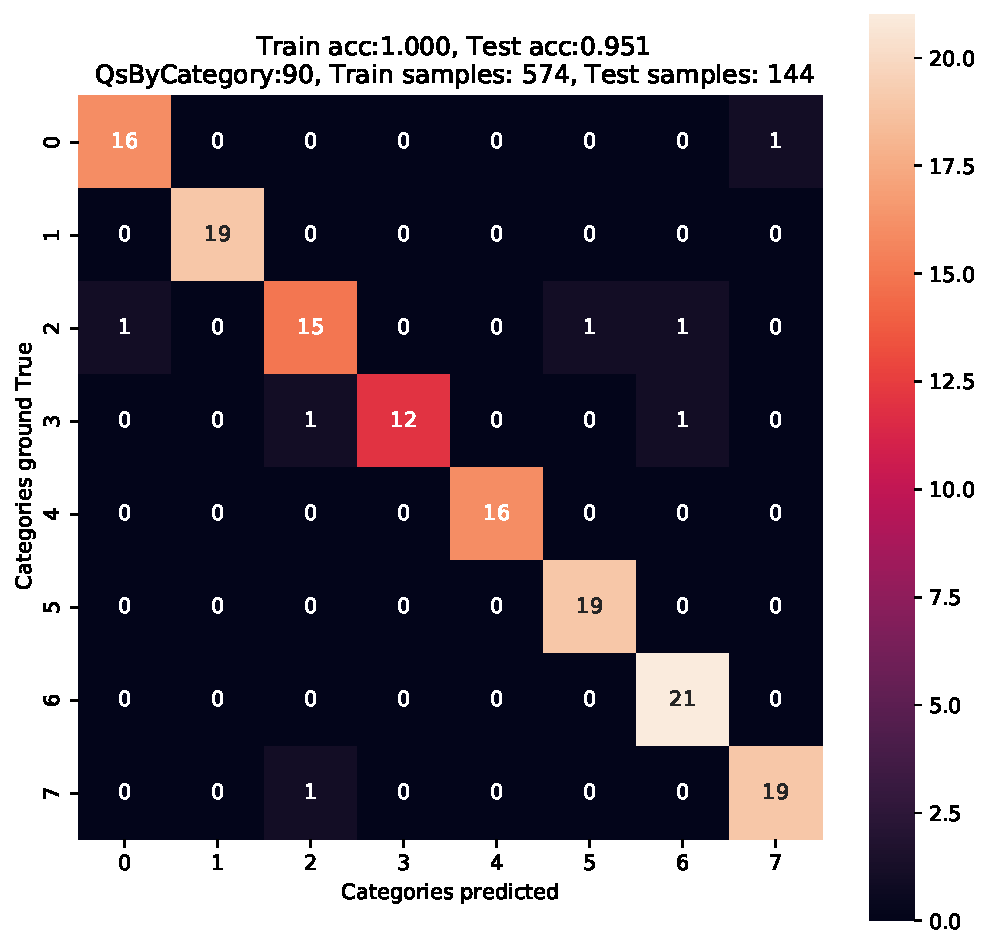
\includegraphics[width=\textwidth]{images/training/training_m1_v2.pdf}
        \caption{Training results of M1: `bert\_base\_uncased + Logistic Regression'.}
        \label{fig:m1}
    \end{minipage}
    %
    \begin{minipage}[c]{0.49\linewidth}
        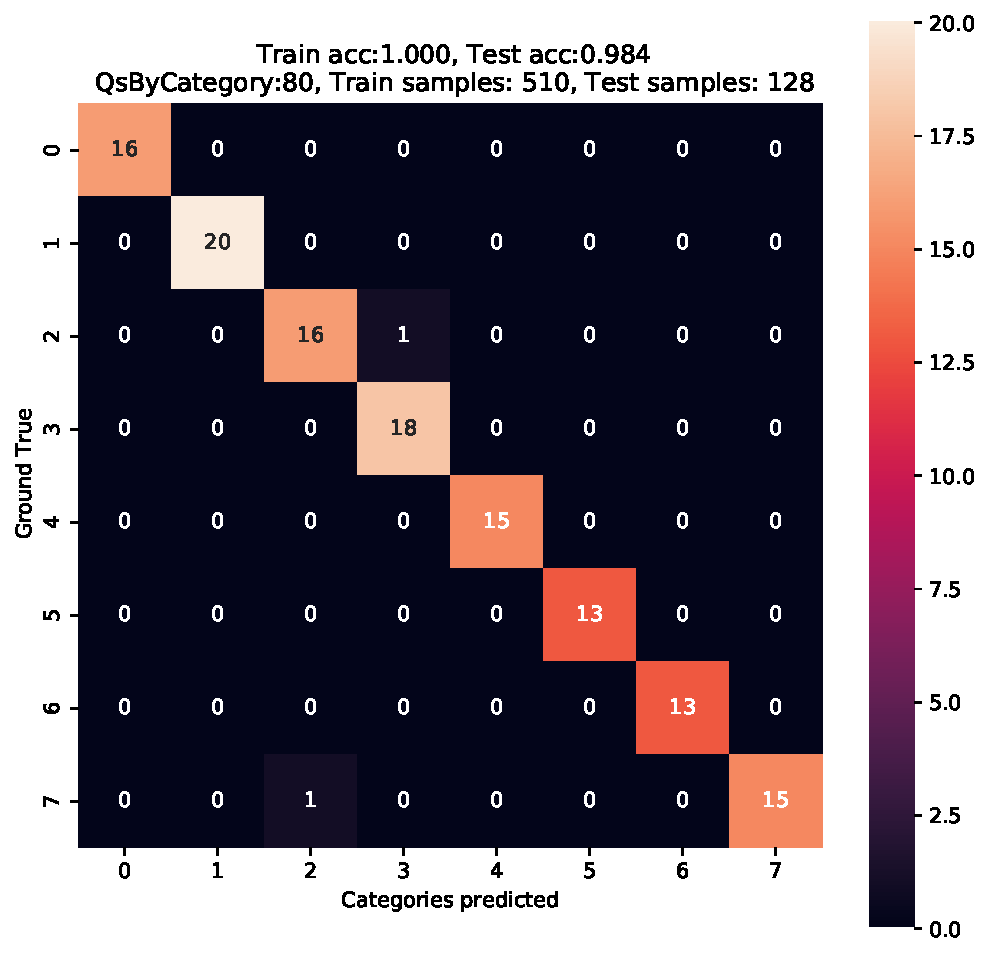
\includegraphics[width=\textwidth]{images/training/training_m2_v2.pdf}
        \caption{Training results of M2: `bert\_base\_uncased + LinearSVC'.}
        \label{fig:m2}
    \end{minipage}
\end{figure}

\begin{figure}[ht!]
    \centering
    \begin{minipage}[c]{0.49\linewidth}
        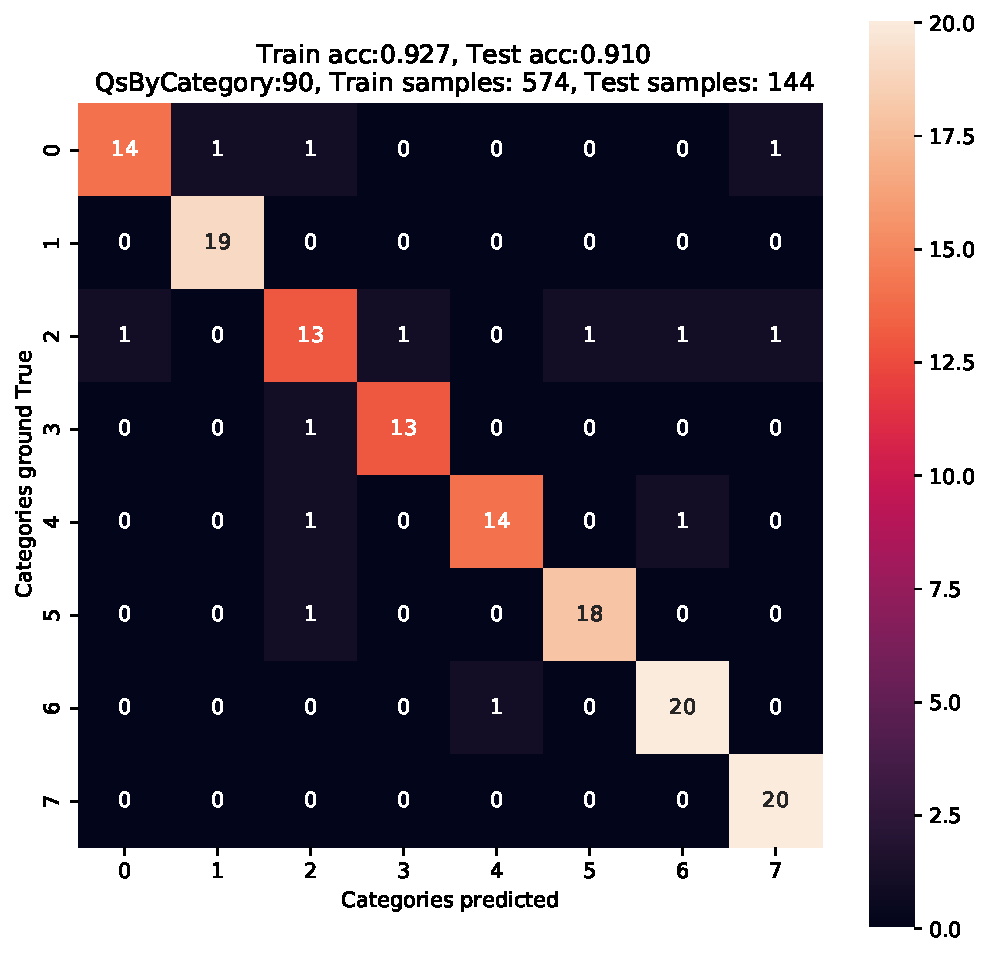
\includegraphics[width=\textwidth]{images/training/training_m3_v2.pdf}
        \caption{Training results of M3: `all-MiniLM-L6-v2 + Logistic Regression'.}
        \label{fig:m3}
    \end{minipage}
    %
    \begin{minipage}[c]{0.49\linewidth}
        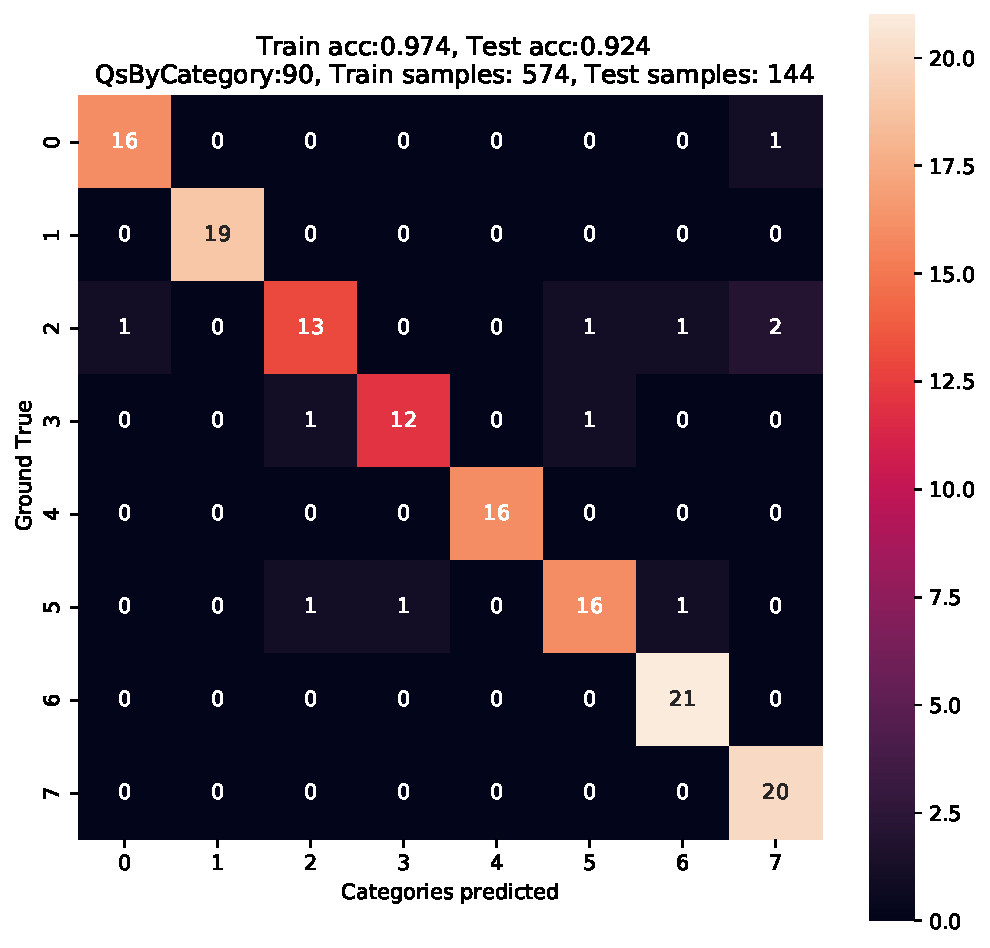
\includegraphics[width=\textwidth]{images/training/training_m4_v2.pdf}
        \caption{Training results of M4: `all-MiniLM-L6-v2 + LinearSVC'.}
        \label{fig:m4}
    \end{minipage}
\end{figure}

% Teniendo en cuenta los resultados anteriores, si bien las cuatro combinaciones lograron buenas precisiones, se observa un leve incremento de rendimiento en aquellas combinaciones que utilizaron \emph{LinearSVC} como modelo de clasificación multi-clase. Por otro lado, al comparar rendimientos en relación a modelos de embedding empleados, las codificaciones con \emph{bert\_base\_uncased } fueron superiores. Esto último, pudiendose atribuir a la mayor cantidad de información contenida en los vectores de dimensionalidad $768$ generados, contra $384$ para \emph{all-MiniLM-L6-v2}. La Figura (\ref{fig:dist_m2}), muestra la distribución de predicciones sobre todas las preguntas de los 17 clusters analizados, utilizando la combinación M2.
Taking into account the previous results, although the four combinations achieved good precision, a slight increase in performance is observed in those combinations that used \emph{LinearSVC} as a multi-class classification model. On the other hand, when comparing performances in relation to the embedding models used, the encodings with \emph{bert\_base\_uncased} were superior. The latter, being attributable to the greater amount of information contained in the generated dimensionality vectors $768$, against $384$ for \emph{all-MiniLM-L6-v2}. The Figure (\ref{fig:dist_m2}), shows the distribution of predictions on all the questions of the 17 analyzed clusters, using the M2 combination.


\begin{figure}[ht!]
    \centering
    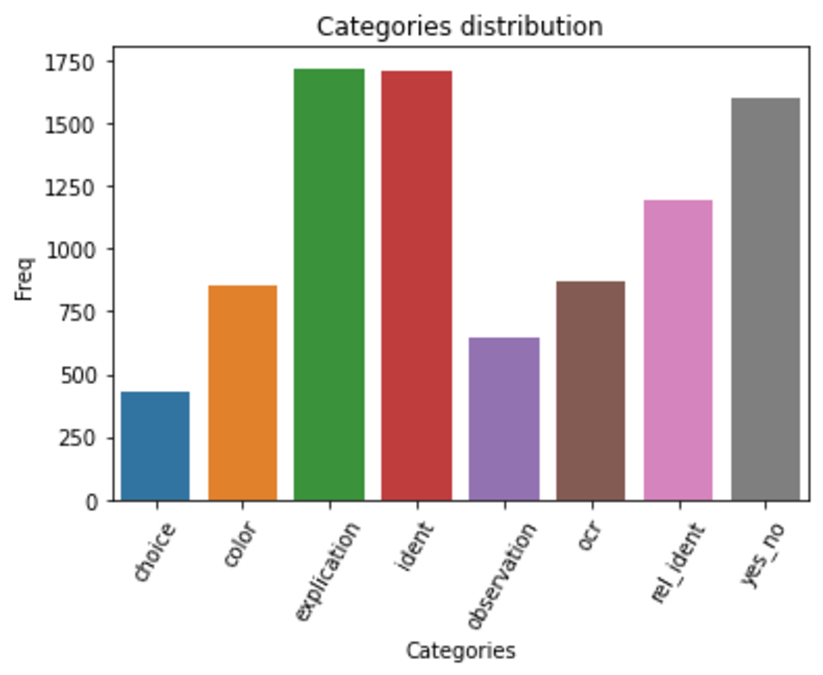
\includegraphics[width=.9\linewidth]{images/training/distribution_m2_v2.pdf}
\caption{Categories distribution using predictions of the models combination M2.}
\label{fig:dist_m2}
\end{figure}